\chapter{User Experience }
\label{cap:user-experience}

\subsection{Il punto di partenza}
Inizialmente, l'applicazione era composta da due sole pagine: una per il wizard in cui l'utente compilava il form di dettaglio del paziente, e una seconda per la visualizzazione dei risultati, dove i grafici erano disposti in una griglia che occupava tutto lo spazio disponibile. Una delle principali carenze del POC iniziale era la mancanza di contesto nei grafici. Questo rendeva difficile la comprensione per utenti senza un background in data science, poiché non potevano interpretare correttamente i dati senza una spiegazione preliminare.\\

Un ulteriore problema riscontrato riguardava la lunghezza del wizard, che inizialmente consisteva di quattro step. Successivamente, un passo è stato eliminato e accorpato al primo per migliorare l'usabilità.

\subsection{Modifiche apportate}

Nella transizione da POC a software completo, il numero di pagine è aumentato: una per il wizard, una per i risultati, una per la valutazione dell'utente e una per il tutorial. Il tutorial è stato posizionato nell'header per garantire un facile accesso da parte dell'utente in qualsiasi momento. Inoltre, il wizard è stato semplificato, eliminando uno step.\\

La pagina dei risultati ha subito le modifiche più significative. È stato inserito un tabbar che permette all'utente di cambiare le visualizzazioni. L'ordine del tabbar è stato progettato in modo tale che l'utente possa vedere prima le singole visualizzazioni e poi tutte insieme in una vista complessiva. Quando si clicca sul tab "All graphs", appare un modale bloccante, che l'utente non può chiudere senza prima compilare il form contenuto al suo interno. Questo form deve essere compilato solo una volta ed è cruciale per raccogliere dati sull'utilità percepita dal medico quando visualizza i vari grafici.\\
È possibile accedere a un altro form tramite il pulsante "Evaluate platform" posizionato in linea con il tabbar. Questo form raccoglie feedback sull'utilità percepita del software nel suo complesso.\\

\begin{figure}[!ht] 
    \centering 
    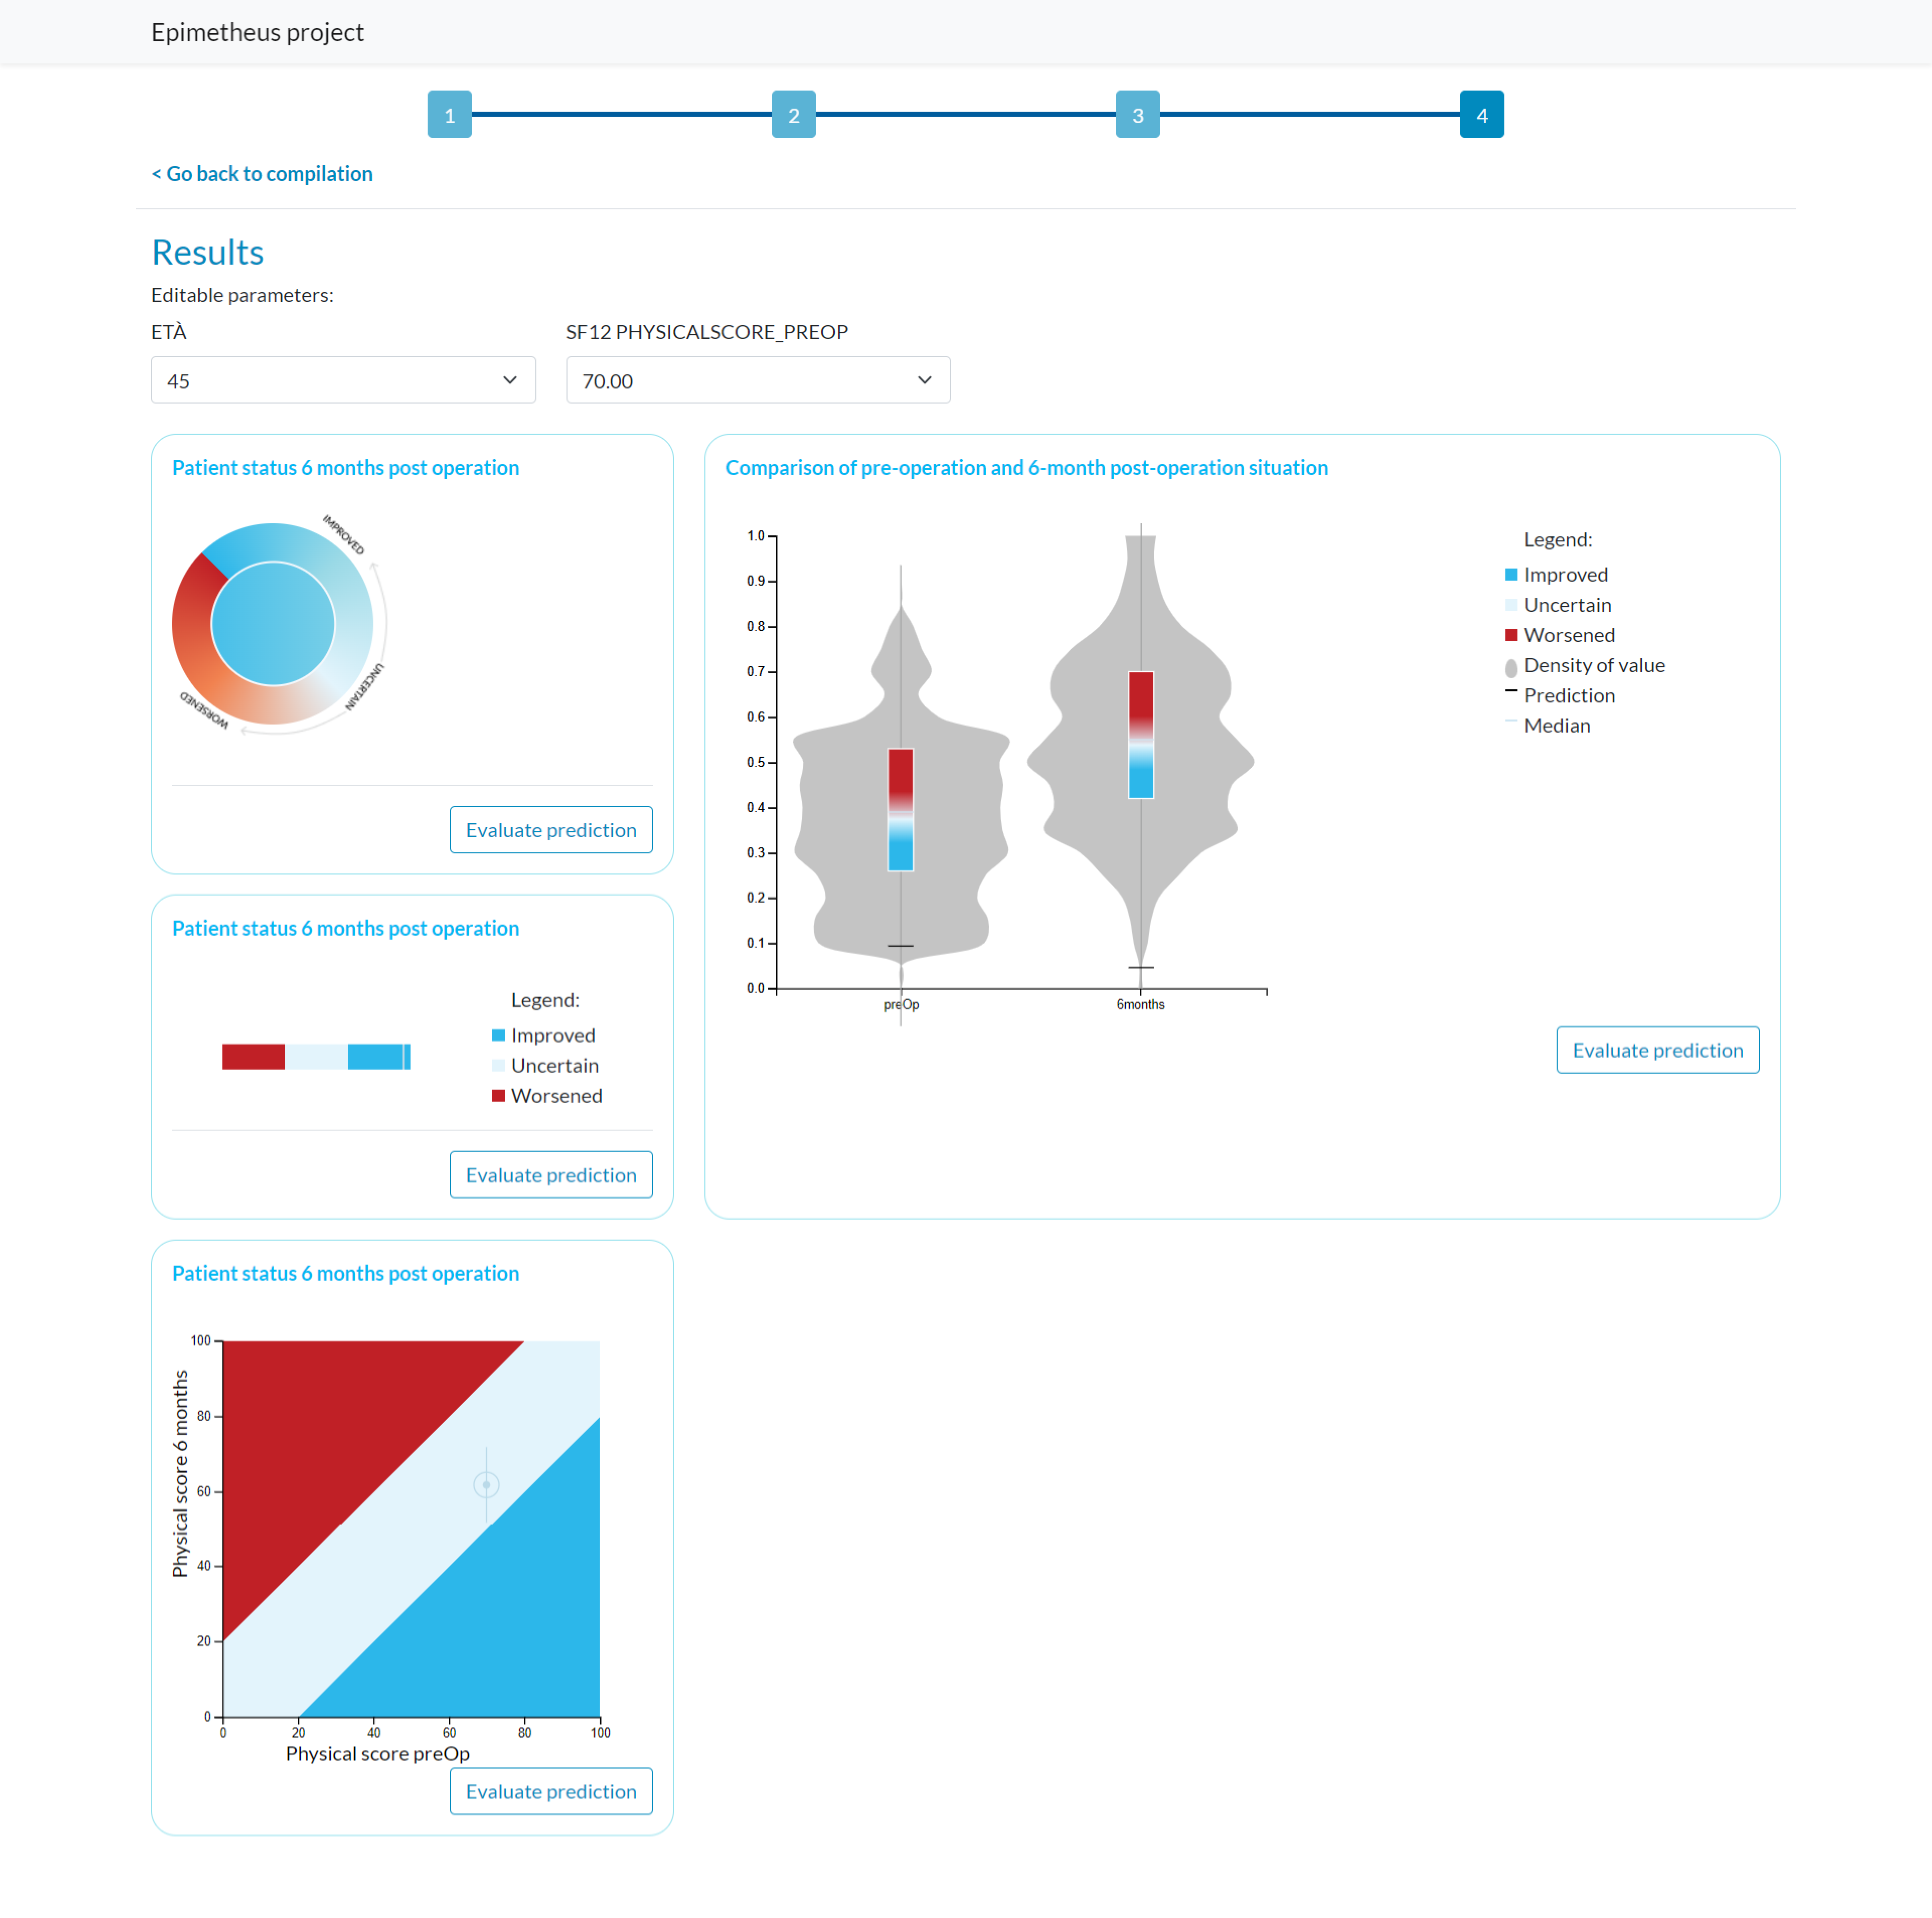
\includegraphics[width=0.9\columnwidth]{epi-start-results} 
    \caption{Pagina di risultati pre-modifiche}
\end{figure}

\begin{figure}[!ht] 
    \centering 
    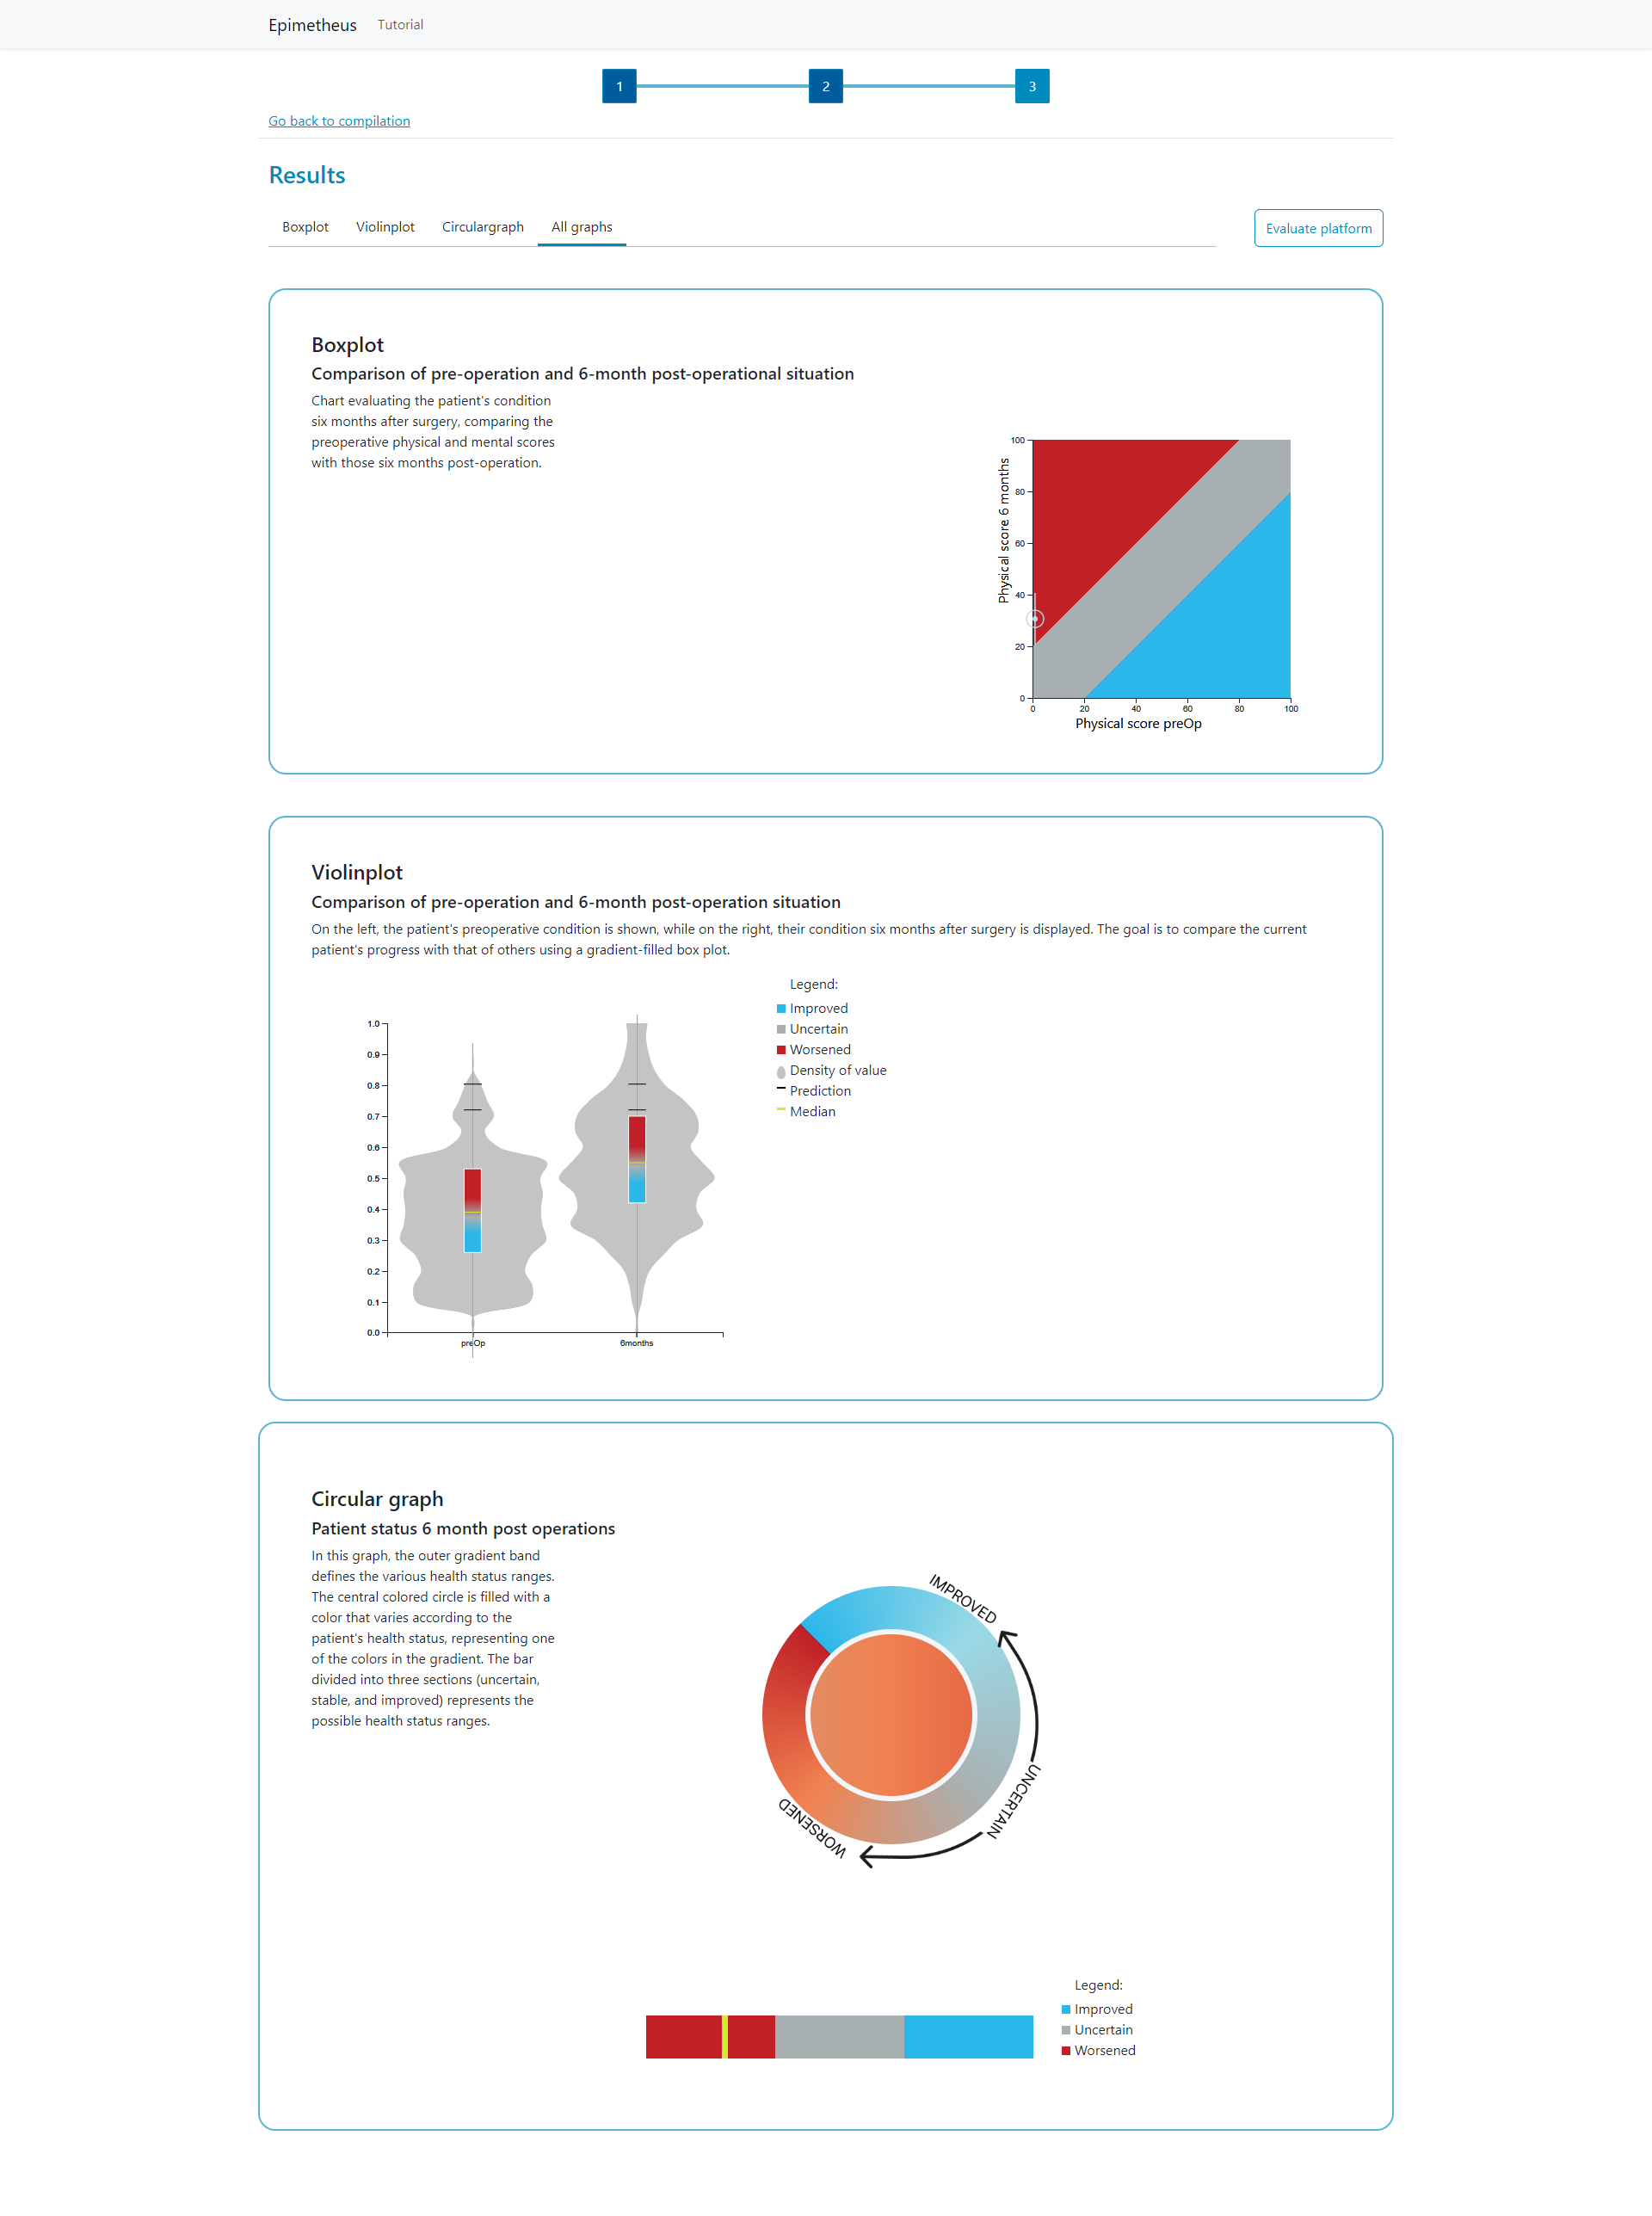
\includegraphics[width=0.9\columnwidth]{epi-all-graphs} 
    \caption{Pagina di risultati post-modifiche}
\end{figure}

I grafici sono interattivi, permettendo all'utente di modificare parametri specifici, come il valore del peso, con conseguente ricalcolo del grafico. Sono state inoltre apportate modifiche ai colori dei grafici. Inizialmente, il colore dell'incertezza era il celeste, ma poiché l'azzurro è il colore primario del brand identity del prodotto, ho deciso di sostituirlo con il grigio. Il grigio, per definizione, si presta meglio a rappresentare il dubbio e l'incertezza. A supporto della mia tesi, test condotti su un campione demograficamente variegato hanno confermato che il grigio è percepito come colore "incerto".\\

Queste modifiche hanno migliorato significativamente l'usabilità e la comprensibilità dell'applicazione, rendendola più intuitiva e user-friendly per gli utenti finali.